\documentclass{article}
\usepackage[utf8]{inputenc}
\usepackage{hyperref}
\usepackage{amsmath}
\usepackage{amsfonts}
\usepackage{amssymb}
\usepackage{braket}
\usepackage{graphicx}

\title{Introduction to Quantum Information and Computing - Notes}
\author{Shrikara A, Arnav Negi, Kriti Gupta, Manav Shah, Muhammed Shamil K,\\ Shiven Sinha, Swayam Agarwal, Vineeth Bhat, Yash Adivarekar, Ayush Acharya} % add contributors
\date{January, 2023}

\begin{document}


\pagenumbering{gobble}
\maketitle
\vfill
\tableofcontents
\newpage
\pagenumbering{arabic}


%fill
\section{Introduction and Motivation}
\subsection{Introduction}

Quantum mechanics is a fundamental theory in physics that provides a description of the physical properties of nature at the scale of atoms and subatomic particles. It is a superset of classical mechanics and can explain
behaviour in experiments that are not explained by only classical mechanics laws. One such experiment is
the Stern Gerlach experiment.\\

The mathematical framework for quantum mechanics is linear algebra. States are described as vectors in a complex
vector space, while measurements and operators are linear operators that act on the space.\\


\subsection{Stern-Gerlach Experiment}

Silver atoms are heated in an oven and projected at a screen through a hole. The stream of silver atoms
are subjected to a homogeneous magnetic field. This causes them to bend in trajectory upwards or downwards.\\

The magnetic moment of the atom is proportional to the spin of the atom's unpaired electron: $\mu \propto S$\\

Because the interaction energy of the magnetic moment with the magnetic field
is just $-\mu \cdot B$ , the z-component of the force experienced by the atom is given by,
$$\textbf{F}_z = \frac{\partial}{\partial z}(-\mu \cdot B) \simeq \mu_z\frac{\partial B_z}{\partial z}$$
The expected pattern is that of a band of silver, however only two spots are observed. This implies
the spin of the atoms along the Z-axis is quantized to two values, $S_z+$ and $S_z-$. This goes against the classical prediction.

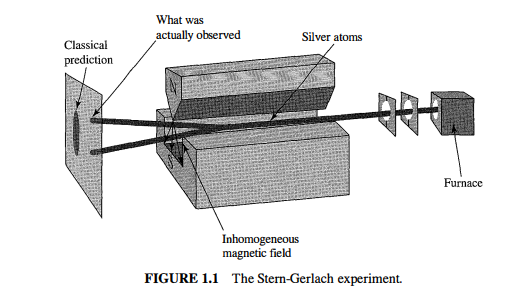
\includegraphics[width = 12 cm]{sterngerlach.png}

Moreover, on sequential Stern-Gerlach experiments, more non classical behaviour was seen.\\

In the experiment, $S_z$ was measured and the atoms with $S_z-$ spin are blocked. Then the rest are
sent through another Stern-Gerlach for measuring $S_x$. Again, the atoms with spin $S_x-$ are blocked.
The final leftover atoms are passed through an experiment measuring $S_z$ again. \\

It is found that even though all atoms with $S_z-$ were blocked, there still are atoms with $S_z-$ spin
after the third experiment. This phenomenon cannot be explained by classical mechanics. Measuring $S_x$ destroys any information obtained about the $S_z$ component of the atoms.

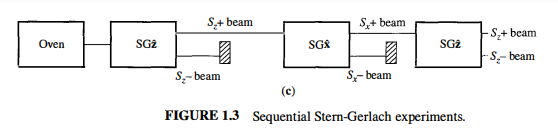
\includegraphics[width = 12 cm]{seqSG.png}

\subsection{Shannon's Theory of Information and Entropy}
Claude Shannon created the modern information theory. He justified use of entropy as measure of information
about a system. The units for information were taken as bits. In terms of quantum information, the units are
qubits. \\

Shannon defined entropy as the average measure of randomness or uncertainty in a system. The Shannon entropy
is defined as entropy H (Greek capital letter eta) of a discrete random variable $X$, which takes values in the alphabet $\mathcal{X}$ and is distributed according to \\

$$p : \mathcal{X} \longrightarrow [0,1]$$ such that $$p(x) := \mathbb{P}[X = x]$$

And H is given by \\
$$H(\mathcal{X}) = \mathbb{E}[-logp(X)] = -\sum_{x \in \mathbb{X}}p(x)logp(x)$$


\subsection{No Cloning Theorem}

In physics, the no-cloning theorem states that it is impossible to create an independent and identical copy of an arbitrary unknown quantum state. This has profound implications in quantum computation. The theorem follows from the fact that all quantum operations must be unitary linear transformation on the state.

\subsection{Outline of the Course}
In the course we will be exploring the following topics:

\begin{enumerate}
	\item Postulates
	\item Everything is a quantum channel
	\item Entanglement, Separability, Non-locality
	\item Teleportation, No Cloning
	\item Entropy, Trace Distance
\end{enumerate}


\section{Finite Dimensional Hilbert Spaces}
A \textit{d}-dimensional Hilbert space $\mathcal{H}$ ($1 \leq d < \infty$) is a complex vector space with an inner product defined on it. A vector in the Hilbert space $\mathcal{H}$ is denoted by $|\psi\rangle $. The inner product $\langle . ,. \rangle : \mathcal{H} \times \mathcal{H} \rightarrow \mathbb{C} $ has the following properties:
\begin{itemize}
	\item \textit{Non negativity -} $\langle \psi , \psi \rangle \geq 0$ $\forall$ $|\psi \rangle \in \mathcal{H}$. $\langle \psi , \psi \rangle = 0$ if and only if $\langle \psi \rangle= 0$.
	      
	\item \textit{Linearity in Second Argument -} $\langle \psi , \alpha \phi_1 + \beta \phi_2 \rangle = \alpha \langle \psi , \phi_1 \rangle + \beta \langle \psi , \phi_2 \rangle $
	      
	\item \textit{Conjugate Linearity in First Argument -} $\langle \alpha \psi_1 + \beta \psi_2 , \phi \rangle = \bar{\alpha} \langle \psi_1 , \phi \rangle + \bar{\beta} \langle \psi_2 , \phi \rangle$
	      
	\item \textit{Conjugate Symmetry -} $\langle \psi , \phi \rangle = \overline{\langle \phi , \psi \rangle}$
\end{itemize}
% continue on isomorphism, standard basis and the inner product <a,b> as a'b  
% Sumeet Khatri and Mark Wilde 

\section{Describing a Closed Physical System}
The complete description of a closed physical system is given by its state $ | \psi \rangle $ where $ | \psi \rangle \in \mathcal{H}$ ($\mathcal{H}$ is a Hilbert Space) and norm of $ | \psi \rangle $ is 1 ($\langle \psi , \psi \rangle = 1$).
For every state $ | \psi \rangle \in \mathcal{H}$, $\exists$ $\langle \psi |$ in the dual vector space of $\mathcal{H}$. Also, $\langle \psi | = (| \psi \rangle)^{\dagger}$.

For $| \psi \rangle$ to represent a closed system, the Hilbert Space it belongs to must have dimension $d \geq 2$, $d \in \mathbb{N}$.

\section{Axioms of Quantum Mechanics}

\subsection{Axiom 1 : Quantum Systems}
A closed quantum system can be represented by its state $| \psi \rangle \in \mathcal{H}$ where $\langle \psi | \psi \rangle = 1$.


\subsection{Axiom 2 : Observables}
Observables are given by Hermitian operators, which take real eigenvalues. (Proven in assignment 1).

\textit{Observables are Linear Operators.} $\hat{O} : \mathcal{H}_1 \rightarrow \mathcal{H}_2$ where $\hat{O}$ is the linear operator denoting the observable.

\textit{Observables are Hermitian.} $\hat{O} = \hat{O}^{\dagger}$

Consider $\psi \in \mathcal{H}_1$, $\phi \in \mathcal{H}_2$.
\begin{equation*}
	\langle \psi , \hat{O} \phi \rangle = \langle \hat{O}^{\dagger} \psi , \phi \rangle
\end{equation*}
In particular, since $\hat{O}$ is Hermitian,
\begin{align*}
	\langle \psi , \hat{O} \phi \rangle = \langle \hat{O} \psi , \phi \rangle \hspace{0.2cm} 
	\forall \psi, \phi                                                                       
\end{align*}
Since $\hat{O}$ is Hermitian, $\mathcal{H}_1$ and $\mathcal{H}_2$ are isomorphic. Also, its eigenvalues are real and distinct eigenvectors are orthogonal(Proved in assignment 1.)\\


Consider the sprectral decomposition of observable $\hat{O}$:
$
\hat{O} = \sum_{a_i} \lambda_i | a_i \rangle \langle a_i|
$
where $|a_i \rangle$s are part of the orthonormal basis. Then
\begin{align*}
	\hat{O}|a_j \rangle & = \sum_{a_i} \lambda_i |a_i \rangle \langle a_i | |a_j \rangle \\
	                    & =\sum_{a_i} \lambda_i |a_i \rangle \delta_{ij}                 \\
	                    & = \lambda_j |a_j \rangle                                       
\end{align*}

\subsection{Aside}
If $\dim \mathcal{H} = d$ and ${|\alpha_1 \rangle , |\alpha_2 \rangle , \ldots , |\alpha_d \rangle}$ is an orthonormal basis,
\begin{align*}
	  & | \psi \rangle = \sum_1^d c_i | \alpha_i \rangle \hspace{0.2cm} ,c_i \in \mathbb{C} \\
	  & \sum_1^d |c_i|^2 = 1                                                                
\end{align*}

WLOG, take $| \alpha_1 \rangle = \begin{bmatrix}
1      \\
0      \\
\vdots \\
0
\end{bmatrix}, |\alpha_2 \rangle = \begin{bmatrix}
0      \\
1      \\
\vdots \\
0
\end{bmatrix} \ldots$ as the standard orthonormal basis and denote them by $|0 \rangle, |1 \rangle , \ldots ,|d-1 \rangle $

For an operator $\hat{A}$, if $\hat{A} \hat{A}^{\dagger} = \hat{A}^{\dagger} \hat{A}$, $\hat{A}|a \rangle = a | a \rangle$, where $a$ is the eigenvalue and $| a \rangle$ is the corresponding eigenvector.

A state $|\psi \rangle$ is of norm 1, i.e. if $| \psi \rangle = \begin{bmatrix}
a_1    \\
a_2    \\
\vdots \\
a_d
\end{bmatrix}$,
$\sqrt{\sum_i |a_i|^2} = 1$


\subsection{Axiom 3 : Measurement}
Measurement $\hat{M}$ corresponding to an observable $\hat{O}$ for any state $| \psi \rangle$ is such that $\hat{M} | \psi \rangle \rightarrow |a_i \rangle$ with outcome $\lambda_i$. After measurement, the final state of the system is one of the eigenstates. Further measurement will produce the same eigenstate and eigenvalue (as long as the repeated measurement is not preceded by the measurement of some other observable.)


A projection matrix $\mathbb{P}$ is a matrix such that $\mathbb{P}^2 = \mathbb{P}$.
$\hat{M}$ is a projection matrix.


\subsection{Axiom 4 : Evolution}
The evolution of quantum states is given by a unitary transformation, ${U : \mathcal{H} \rightarrow \mathcal{H}}$ where $U^{\dagger}U = UU^{\dagger} = \mathbb{I}$

\section{Multiple Systems}
Let $H_{A}$ and $H_B$ be two system. To visualize multiple systems as a single system we use the idea of tensor product.\\
$H_A \otimes H_B$ denotes the tensor product of $H_A$ and $H_B$\\
For e.g. consider the following example : \\ \newline
\[
\begin{bmatrix}
	a_{11} & a_{12} \\
	a_{21} & a_{22} 
\end{bmatrix}
A = \begin{bmatrix}
a_{11}A & a_{12}A \\
a_{21}A & a_{22}A
\end{bmatrix}\\
\]

We can easily see that
\begin{align*}
	dim(H_A \otimes H_B) = dim(H_A)\times dim(H_B) 
\end{align*}
\section{Noisy Quantum Theory}
Expectation value of an observable A is
\begin{align*}
	<A>_{\psi} = <\psi|A|\psi> 
\end{align*}
If $\psi$ is not normalized then normalize it by dividing with $<\psi|\psi>$.\\
Now even if I change $|\psi>$ to $e^{\iota\phi}|\psi>$ expectation value does not changes because \\
\begin{align*}
	<\psi|e^{-\iota\phi} A e^{\iota\phi}|\psi> = <\psi|A|\psi>  \tag*{($e^{\iota\phi}$ is just a scalar)} 
\end{align*}
\section{Density Operator}
A quantum state is represented by a density operator defined on a  \\
Hilbert space H. \\
\begin{center}
	\( \rho : H \rightarrow H\)
\end{center}
\subsection{Requirement of Density operator}
The question arises that what's the need of representing a state in terms of density operator. \\
State vectors or wave functions $(|\psi>)$ can only represent pure states. Density operator can also represent mixed state. \\
Density operator also allows for the calculation of the probabilities of the outcomes of any measurement performed upon system, using the Born rule.
\subsection{Properties of Density operator}
\begin{itemize}
	\item \(\rho \geq 0\) \\
	      This means that all the eigenvalues of $\rho$ are $\geq 0$
	\item \(\rho = \rho^\dagger\) \\
	      $\rho$ should be a Hermitian-matrix
	\item $Tr(\rho) = 1$ \\
	      The summation of the diagonal elements of $\rho = 1$
\end{itemize}
So summarising, Density operator for a system is a positive semi-definite, Hermitian operator of trace one acting on the Hilbert space of the system
\newline \newline
For any state $|\psi>$, its density operator is $|\psi><\psi|$.\\
Let's prove that $|\psi><\psi|$ follows all the property of the density operator : \\
\newline
We know that $(|\psi><\psi|)^2 = |\psi><\psi|\psi><\psi| = |\psi><\psi|$ \\
So it's clear that $|\psi><\psi|$ is a pure state $\implies$ all eigenvalues are $\ge$ 0.\\ So first property is satisfied. \\
\begin{flushleft}2\end{flushleft}
\begin{align*}(|\psi><\psi|)^\dagger & = (<\psi|)^\dagger (|\psi>)^\dagger \\
	  & = |\psi><\psi| 
\end{align*}
Hence $<\psi|\psi>$ is a hermitian operator.\\
\newline
3. \begin{align*}
Tr(|\psi><\psi|) & = Tr(<\psi|\psi>)  \tag*{(Trace Theorem)} \\
& =1
\end{align*}
Hence, the trace of $|\psi><\psi| = 1$.\newline
All the properties are satisfied by $|\psi><\psi|$.

\section{Observables}
\begin{itemize}
	\item Each observable can be represented by Hermitian operators.
\end{itemize}
\begin{itemize}
	\item Expectation value of an observable ${\hat{O}}$ for a quantum state $\rho$  is Tr[${\hat{O}\rho}$]
\end{itemize}
\begin{itemize}
	\item If $\rho$ is pure state {$\{|\psi\rangle\langle\psi|\}$}, then:\\\\
	      Tr[${\hat{O}\rho}$]=Tr[${\hat{O}|\psi\rangle\langle\psi|}$]=Tr[${\langle\psi|\hat{O}|\psi\rangle}$]=${\langle\psi|\hat{O}|\psi\rangle}$
\end{itemize}
\begin{itemize}
	\item If $\rho$ is not a pure state, i.e., $\rho$=$\sum\limits_{i}p_{i}|\psi_{i}\rangle\langle\psi_{i}|$, then:\\\\
	      Tr[${\hat{O}\rho}$]=Tr[${\hat{O}\sum\limits_{i}p_{i}|\psi_{i}\rangle\langle\psi_{i}|}$]=$\sum\limits_{i}p_{i}$Tr[${\hat{O}|\psi_{i}\rangle\langle\psi_{i}|}$]=$\sum\limits_{i}p_{i}\langle\psi|\hat{O}|\psi_{i}\rangle$
	      
\end{itemize}

\section{Mixed State}
Mixed state is said to be the mixture of the different pure states.\\
Mixed states can be written as:
$\sigma=\sum\limits_{i}p_{i}\rho_{i} , where \sum\limits_{i}p_{i}=1$\\
Here $\sigma$: is the mixed state , $\rho_{i}$:pure state and $p_{i}$: probability of state $\rho_{i}$ to be present in the mixed state.
\begin{itemize}
	\item A state is pure if $\rho^2=\rho$
\end{itemize}
Example1:-
Let us consider a system which has 5 qubits of $|0\rangle$ and 5 qubits of $|1\rangle$ where $\{|0\rangle,|1\rangle\}$ are orthonormal basis. Find the mixed state of the system.\\
Answer1:- $\sigma=\frac{1}{2}\{|0\rangle\langle0|+|1\rangle\langle1|\}$\\\\
Example2:-
Let us consider a system which has 5 qubits of $|+\rangle$ and 5 qubits of $|-\rangle$ where $\{|+\rangle,|-\rangle\}$ are orthonormal basis. Find the mixed state of the system.\\
Answer2:- $\sigma=\frac{1}{2}\{|+\rangle\langle+|+|-\rangle\langle-|\}$\\\\
Note:- Both $\sigma$ obtained in the above two examples are one and the same.\\
Proof:-\\
$\sigma=\frac{1}{2}\{|0\rangle\langle0|+|1\rangle\langle1|\}=\frac{1}{2}\{|+\rangle\langle+|+|-\rangle\langle-|\}$\\\\
$\sigma$=$\frac{1}{2}(\sum\limits_{i}|i\rangle\langle i|)$=$\frac{1}{2}(\sum\limits_{i}|i\rangle\langle i|)$\\\\
$\sigma=\frac{1}{2}\mathbb{1}=\frac{1}{2}\mathbb{1}$

\section{Superposition}
The linear combination of states is called superposition.\\
A superpositioned state can be represented as:\\
$|\psi\rangle=\sum\limits_{i}c_{i}|\psi_{i}\rangle$,\\
where $\sum\limits_{i}c_{i}^2=1$ and $|\psi_{i}\rangle$ are the states that are being superimposed.

\section{Measurements}
The most general kind of measurements are called POVM’s. POVM stands for positive operator valued measure. \\
They are denoted by \{$\Lambda^{x}$\}$_{x}$. It is a collection of positive semi-definite operators such that: \\ \\
{$\Lambda^{x}$} $\ge$ 0 and $\sum\limits_{x}$ {$\Lambda^{x} = 1$}. \\

\subsection{Projective Measurements}
They are denoted by $\{\mathbb{P}_{x}\}$. They are POVMs with additional properties:
\begin{itemize}
	\item $\mathbb{P}_{i}^{2} = \mathbb{P}_{i}$
\end{itemize}
\begin{itemize}
	\item $\mathbb{P}_{i} \mathbb{P}_{j}  = \delta_{ij} \mathbb{P}_{i} = \delta_{ij} \mathbb{P}_{j}$
\end{itemize}
where $\mathrm{x}$ is the outcome of the measurement and $\mathbb{P}_{i}$, $\mathbb{P}_{j} \in \mathbb{P}_{x}$ \\ \\

\section{Measurement Probability}
\subsection{Born's Rule}
The Born's Rule is a postulate of Quantum Mechanics which helps determine the probability that a measurement of a quantum system will yield a given result. \\ \\
The Born's rule states that if an observable corresponding to a self-adjoint operator A with discrete spectrum is measured in a system with normalized wave function
$|\psi \rangle$ then:

\begin{enumerate}
\item The measured value will be one of the eigenvalues $\lambda$ of A.
\item The probability of measuring a given eigenvalue $\lambda_{i}$ will be equal to
${\displaystyle \langle {\psi} |P_{i}| {\psi} \rangle }$ where $P_{i}$ is the projection onto the eigenspace of A corresponding to $\lambda_{i}$.
Equivalently, the probability can be written as $|\langle \lambda _{i}|\psi \rangle |^{2}$
where $|\lambda_{i} \rangle$  is the eigenvector associated with the eigenvalue $\lambda_{i}$.
\end{enumerate}
\subsubsection{POVM Version of Born's Rule}
The POVM element ${\displaystyle F_{i}}$ is associated with the measurement outcome ${\displaystyle i}$, such that the probability of obtaining it when making a measurement on the quantum state ${\displaystyle \rho }$  is given by:

$${\displaystyle p(i)=\operatorname {tr} (\rho F_{i})}$$

The measurement of a quantum system in the state $\rho$ according to the POVM
$M_{x} : x \in X$ induces a probability distribution. This distribution takes values belonging to the set of all possible values of $x$, and is defined by the Born rule:

$$ p(x) = Tr[M_{x} \rho] $$

To determine the post-measurement states of the system being measured:
\\
Taking measurement with a projective operator $\mathbb{P}_{i}$.
In this case let the post-measurement state be $\rho^{x}$.


\begin{align*}
	\rho &\xrightarrow{\mathbb{P}_{i}} \rho '\\
	\rho' &= \dfrac{\mathbb{P}_{i} \rho \mathbb{P}_{i} ^ \dagger}{Tr[{\mathbb{P}_{i} \rho \mathbb{P}_{i} ^ \dagger}]}
\end{align*}
Set of Orthonormal Basis is a projective measurement because it satisifes POVM and also the projective measurement conditions.
\\
After measuring once if we measure the same observable again , it will return the same outcome.
\\
Proof:
Assume we got outcome as $\mathrm{i}$ in our first measurement. From previous our new state is $\rho '$.
\\
\begin{align*}
p(i) &= Tr \left[\mathbb{P}_{x}\rho ' \right] \\
	&= Tr \left[\mathbb{P}_{x} \dfrac{\mathbb{P}_{i} \rho \mathbb{P}_{i} ^ \dagger}{Tr\left[{\mathbb{P}_{i} \rho \mathbb{P}_{i} ^ \dagger}\right]}\right] \\
	&= Tr \left[\dfrac{\delta_{xi} \mathbb{P}_{i} \rho \mathbb{P}_{i} ^ \dagger}{Tr\left[{\mathbb{P}_{i} \rho }\right]}\right]
\end{align*}
\\
This value clearly would be 1 in case $x = i$ otherwise this will be equal to 0.
\\
Hence Proved.

\section{Transformation/Evolution of Quantum States}

Quantum Communication necessarily involves the evolution
of quantum systems (such as the evolution of photons when travelling through
an optical fiber). Mathematically, this evolution is described by a
quantum channel.
\\
\\
A Quantum channel is a linear, completely positive, and trace-preserving map acting on the state of the system. Note that we are working with Open Quantum Systems while talking about Quantum Channels.
\\
\[\mathcal{N}_{A \rightarrow B} : \mathcal{B}(\mathcal{H}_{A}) \rightarrow \mathcal{B}(\mathcal{H}_{B})\]
Note: $\mathcal{B}(\mathcal{H}_{A})$ denotes the set of operators.
$dim(\mathcal{H}_{A})$ need not be equal to $dim(\mathcal{H}_{B}.)$
\\
\\
Introduction to Trace Preserving and Completely Positive properties:
\\
New density operator also has trace equal to 1 and the channel produces a semi-definite state as output always if the choi of the channel is $\ge$ 0.
\\
\\
Everything is a Quantum Channel with respect to time.

\section{Quantum Channel}
\[
	\mathcal{N}_{A \rightarrow B} : \mathcal{B}(\mathcal{H}_{A}) \rightarrow \mathcal{B}(\mathcal{H}_{B})
\]

where
\begin{align*}
	(\mathcal{H _{A}}) &= \text{Hilbert space of input system} \\
	(\mathcal{B}) &= \text{Set of bounded operators}
\end{align*}
Quantum channel is trace-preserving since it maps trace-class operators to trace-class operators.
\\
\small
A matrix with a finite trace represents a trace-class operator.
A finite-dimensional matrix is a trace-class operator if it is bounded.
\\
\normalsize
A \textbf{Super Operator} acts on an operator to give an operator.

\subsection{Properties of Quantum Channel}
For a super operator to be a quantum channel, it has to follow the following properties:
\begin{enumerate}
	\item Completely positive
	      \begin{gather*}
	      	id_{B} \otimes \mathcal{N}_{A \rightarrow{} C} (\Phi_{AB}) \geq 0
	      \end{gather*}
	      where $\Phi _{AB}\geq 0$ and $id$ = identity super operator, and $\phi_{AB}$ is a maximally entangled state.
	      
	      \subitem Positivity:
	      $X_{A} \geq 0 \Rightarrow{} \mathcal{N}_{A\rightarrow{} C} (\mathcal{X}_{A}) = \mathcal{Y}_{C} \geq 0$
	      
	\item Trace-preserving map
	      \begin{gather*}
	      	Tr[\rho_{A}] \Rightarrow{} Tr[\mathcal{N}_{A \rightarrow C} (\rho _{A})]
	      \end{gather*}
\end{enumerate}

\section{Joint States}
\subsection{Product State}
The density operator of the product state of A and B is the tensor product of the density operators of A and B.
\begin{gather*}
	\rho _{AB} = \rho _{A} \otimes \sigma _{B}
\end{gather*}
In a product state, there is no correlation between the two states. A and B are independent.

\subsection{Separable States}
The density operator of a separable state is obtained as:
\begin{gather*}
	\rho _{AB} =  \sum_{x} p_{x} \rho ^{(x)} _{A} \otimes \sigma ^{(x)} _{B}  \\
\end{gather*}
where $p _{x}$ is the probability of each state such that
\begin{gather*}
	\sum p_{x} = 1,   p_{x} \geq 0
\end{gather*}
Here, $\rho ^{(x)} _{A} $ and $\sigma ^{(x)} _{B}$ may be pure or mixed states.

\subsection{Entangled State}
State which cannot be written as separable states or product of states is in an entangled state.
\begin{gather*}
	\mathcal{N}_{A \rightarrow C}(\Phi _{AB})
\end{gather*}
Dimension, d = $min(dim(\mathcal{H}_{A}), dim(\mathcal{H}_{B}))$\\

Maximally entangled state: $\Phi_{AB} = \frac{1}{d} \sum_{i,j=0}^{d-1}\ket{i}_{A} \otimes \ket{i}_{B} \bra{j}_{A} \otimes \bra{j}_{B}\\
=\frac{1}{d} \sum_{i,j=0}^{d-1}\ket{i} \bra{j}_{A} \otimes \ket{i} \bra{j}_{B}
$

\section{Kraus Operators: $K_{i}$}
\begin{gather*}
	\mathcal{N}_{A \rightarrow C} (\cdot) = \sum_{i} K_{i}(\cdot) K_{i}\textsuperscript{\textdagger}
\end{gather*}
where
\begin{gather*}
	\sum K_{i}\textsuperscript{\textdagger} K_{i} =  \mathbb{1}\\
	K_{i} : \mathcal{H}_{A} \rightarrow{} \mathcal{H}_{C}
\end{gather*}

For any completely positive, trace-preserving quantum channel, $\exists$ Kraus operators.

If an $\mathcal{N}$ has Kraus operators $\Rightarrow{}$ it is completely positive and trace-preserving.
\\\\
Projective measurement is a special case of quantum channel where $\mathbb{P}$s are Kraus operators.
\section{Recapitulation of Quantum Channels}

A quantum channel $\mathcal{N}_{A \rightarrow B}$ taking operators from the set of bounded operators in $A$ to the set of bounded operators in $B$ is defined as

\[\mathcal{N}_{A \rightarrow B} : \mathcal{B}(A) \rightarrow \mathcal{B}(B)\]

has the following properties:

\subsection{Trace Preserving}

\[\forall X \in \mathcal{B}(A),\quad Tr(\mathcal{N}_{A \rightarrow B}(X))=Tr(X) \]

This preserves the validity of the outcome of the operation by keeping the trace as $1$.

\subsection{Completely Positive}

Taking the maximally entangled state $\Phi_{RA}$, defined as

\[\Phi_{RA} = | \phi \rangle \langle \phi | _{RA}\]

where the system $R$ is a space characteristic of the channel, and,

\[| \phi \rangle _{RA} = \frac{1}{\sqrt{d}}\ \Sigma^{d-1}_{i=0} | i \rangle_R | i \rangle_A \]

where

\[ \{| i \rangle_R \}_i \quad \textrm{forms an orthonormal basis of R} \]
\[ \{| i \rangle_A \}_i \quad \textrm{forms an orthonormal basis of A} \]
\[d = infinum\{ dim(A), dim(R)\}\]

the channel produces a semi-positive definite state as output regardless of input if

\[ \mathcal{N}_{A \rightarrow B}(\Phi_{RA}) 	\geq 0 \]

Here, $\mathcal{N}_{A \rightarrow B}(\Phi_{RA})$ is referred to as the \emph{Choi} of the channel.

\section{Pure States}

Pure states can be represented by $| \phi \rangle _{RA}$ such as:

\[| \phi \rangle _{RA} = \Sigma^{d-1}_{i=0} \sqrt{p_i}| i \rangle_R | i \rangle_A \]

where $d$, $| i \rangle_R$ and $| i \rangle_A$ remain the same as defined in the recapitulation.

$p_i$ represents the probability of $| i \rangle_R | i \rangle_A$ in the superposition of states, and $\Sigma^{d-1}_{i=0} {p_i} = 1$.

\noindent Further, if the number of basis vectors in $R$ exceeds $d$ then we can choose any $d$ arbitrary basis vectors for forming
$\{| i \rangle_R \}_i$

\section{Further comments}

\begin{description}
	
	\item It must be noted that we are working in an \emph{open quantum system} while working with quantum channels
	
	\item Also,
	\[ \mathcal{N}_{A \rightarrow B}(\varphi_A) = Tr_{_{E'}}[U_{AE \rightarrow BE'} (\varphi_A \otimes \omega_E) U_{AE \rightarrow BE'}^{\dagger} ]\]
	
	where $U_{AE \rightarrow BE'}$ is a unitary matrix. Now, unitary matrices are square matrices implying that their application on a matrix preserves the matrix's dimensions. So, we have
	
	\[dim(AE) = dim(BE')\]
	
	$Tr_{_{E'}}(.)$ is the partial trace of $(.)$ with respect to matrix $E'$ defined as
	
	\[ Tr_{_{B}}(X_{AB}) = \Sigma_i \langle i |_{B} X | i \rangle_{B} \]
	
	where $\{ | i \rangle_{B} \}_i$ forms the orthonormal basis of $B$.
	
	The partial trace with respect to $B$ trims the input $X_{AB}$ to a matrix $Y_A$ in $A$ by removing all indication of $B$.
	
	\item $M_A \otimes N_B (\varphi_{AB})$  is a \emph{local operation} on $\varphi_{AB}$ where $M_A$ acts on $A$ and $N_B$ acts on $B$. Moreover,
	
	\[ [ M_A \otimes \mathcal{I}_B, \mathcal{I}_A \otimes N_B ] = 0 \]
	
	which indicates that the order of application of $M_A$ and $N_B$ on $\varphi_{AB}$ doesn't matter.
	
	\item We also note
	
	\[ Tr_{_A}[M_A \otimes N_B (\varphi_{AB})] = N_B(\varphi_B) \]
	
	where
	
	\[ \varphi_B = Tr_{_A}[\varphi_{AB}] \]
	
\end{description}

\end{document}